\section{Phiên bản sản phẩm tối thiểu khả thi - MVP}

Dưới đây là User Interface ban đầu của Mutux mà nhóm sẽ thiết kế MVP.

\begin{figure}[H]
    \centering
    
    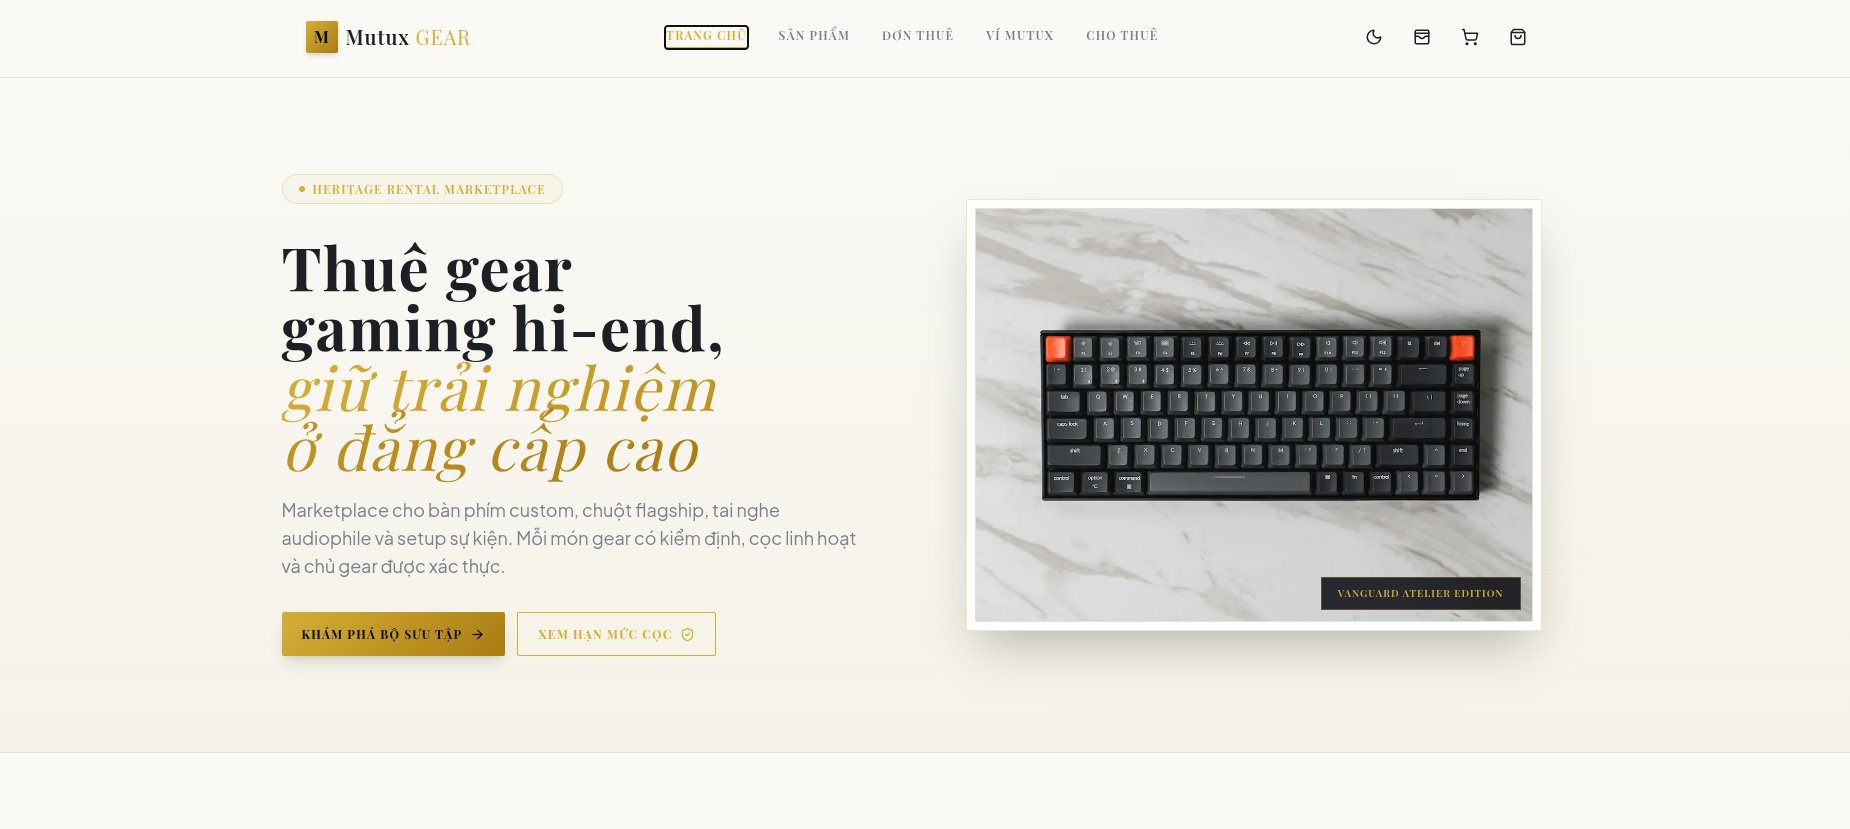
\includegraphics[width=1\textwidth]{PA2/img/mvp/frontpage1.png}
    
    \caption{Trang chủ của Mutux}
    \label{fig:my_image} 
\end{figure}

Từ landing page này, người dùng có thể xem qua và tìm hiểu về Mutux.

\begin{figure}[H]
    \centering 
    
    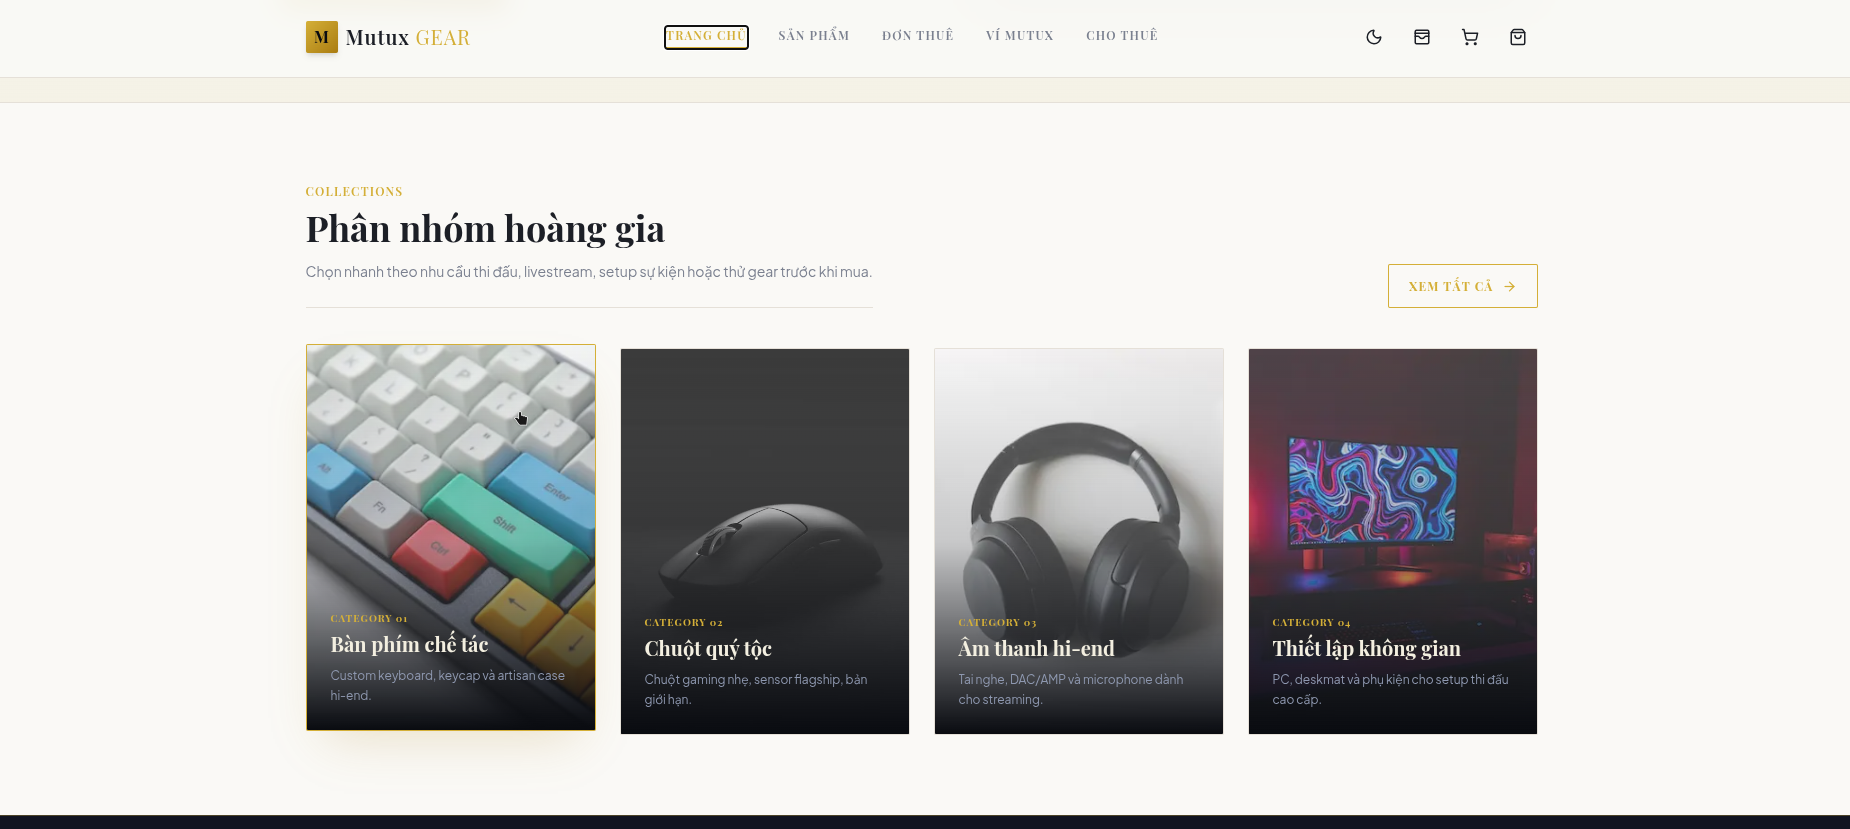
\includegraphics[width=1\textwidth]{PA2/img/mvp/frontpage2.png}
    
    \caption{Trang chủ của Mutux}
    \label{fig:my_image}
\end{figure}

\begin{figure}[H]
    \centering 
    
    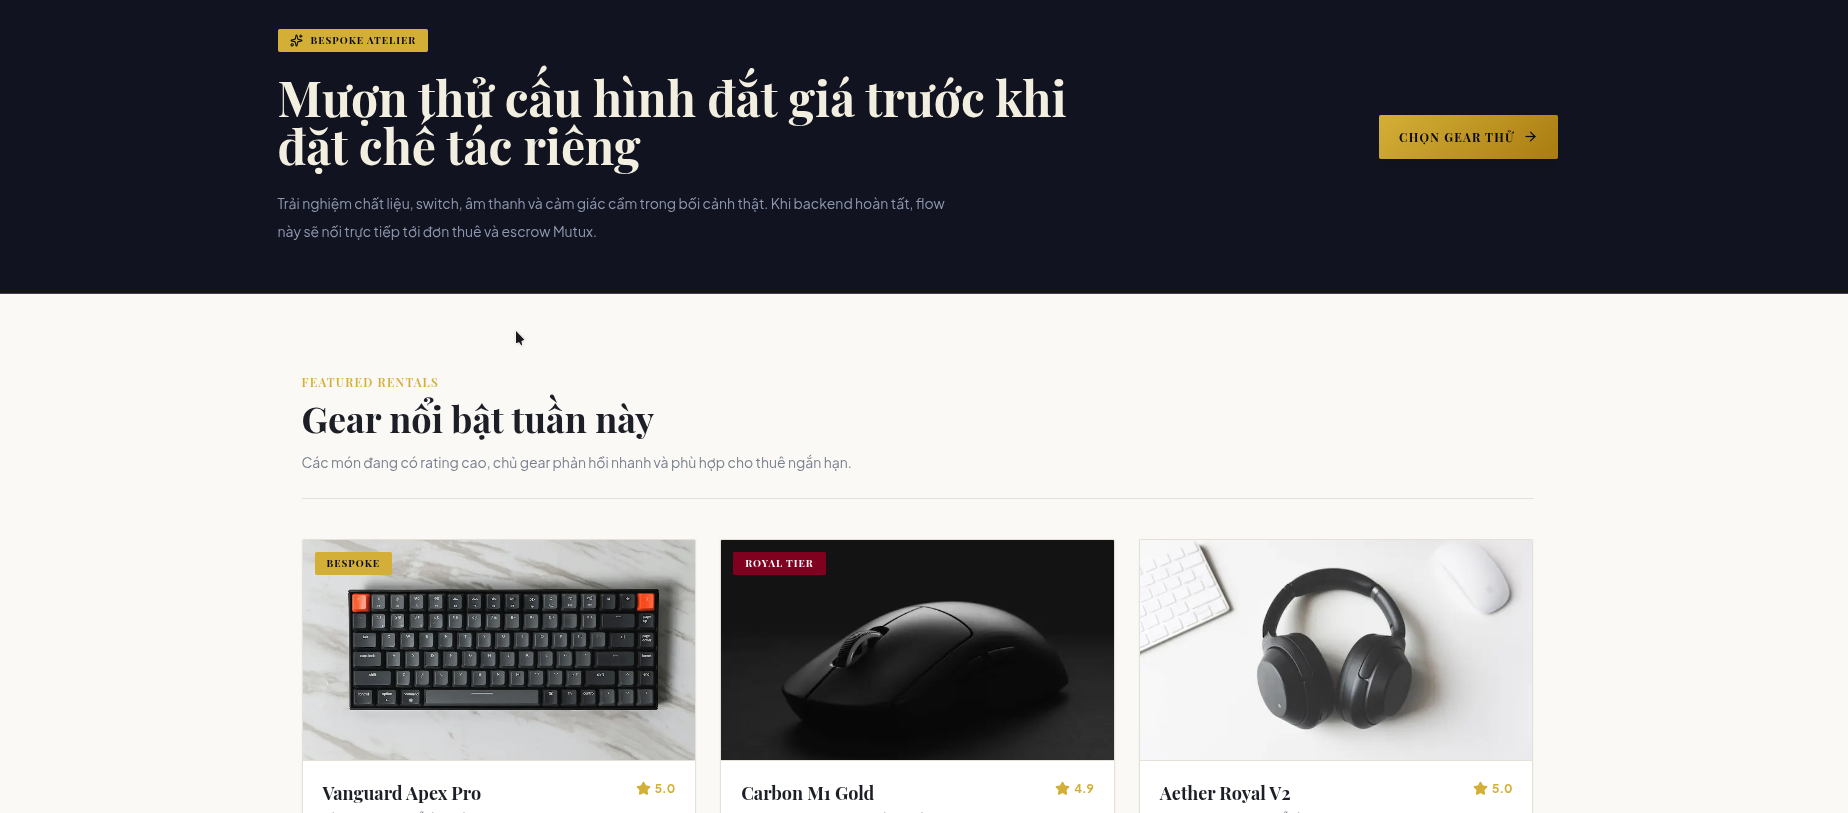
\includegraphics[width=1\textwidth]{PA2/img/mvp/frontpage3.png}
    
    \caption{Trang chủ của Mutux}
    \label{fig:my_image}
\end{figure}

\begin{figure}[H]
    \centering 
    
    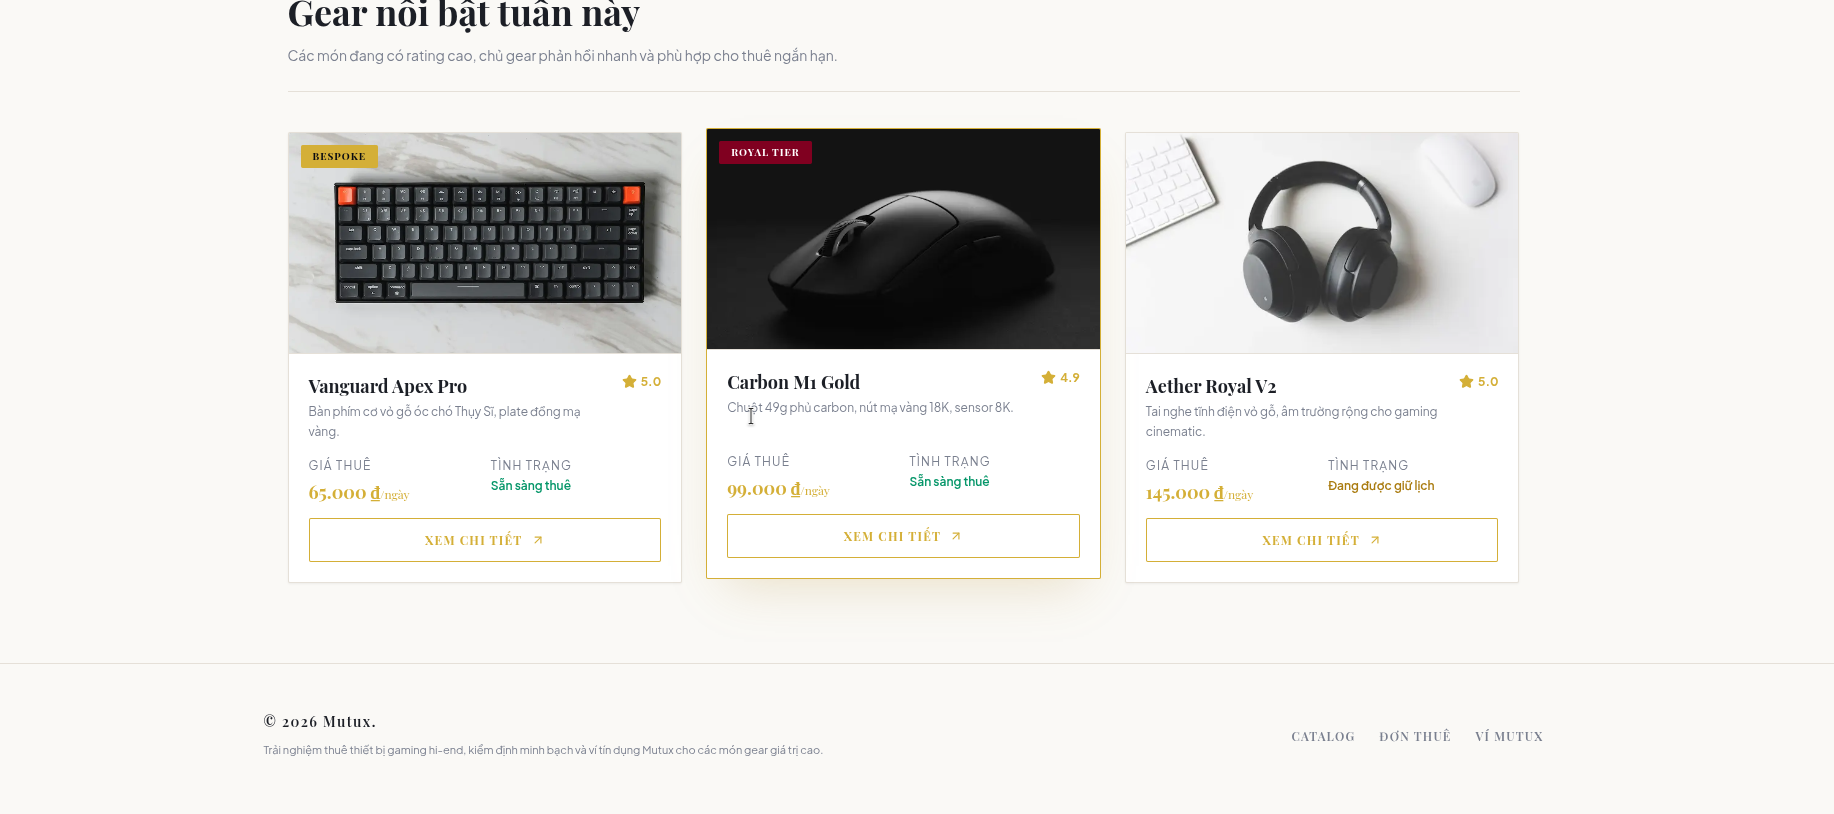
\includegraphics[width=1\textwidth]{PA2/img/mvp/frontpage4.png}
    
    \caption{Trang chủ của Mutux}
    \label{fig:my_image}
\end{figure}

Tiếp đến, người dùng có thể vào mục \textbf{Sản phẩm} để xem danh mục các sản phẩm đang được cho thuê trên sàn.


\begin{figure}[H]
    \centering 
    
    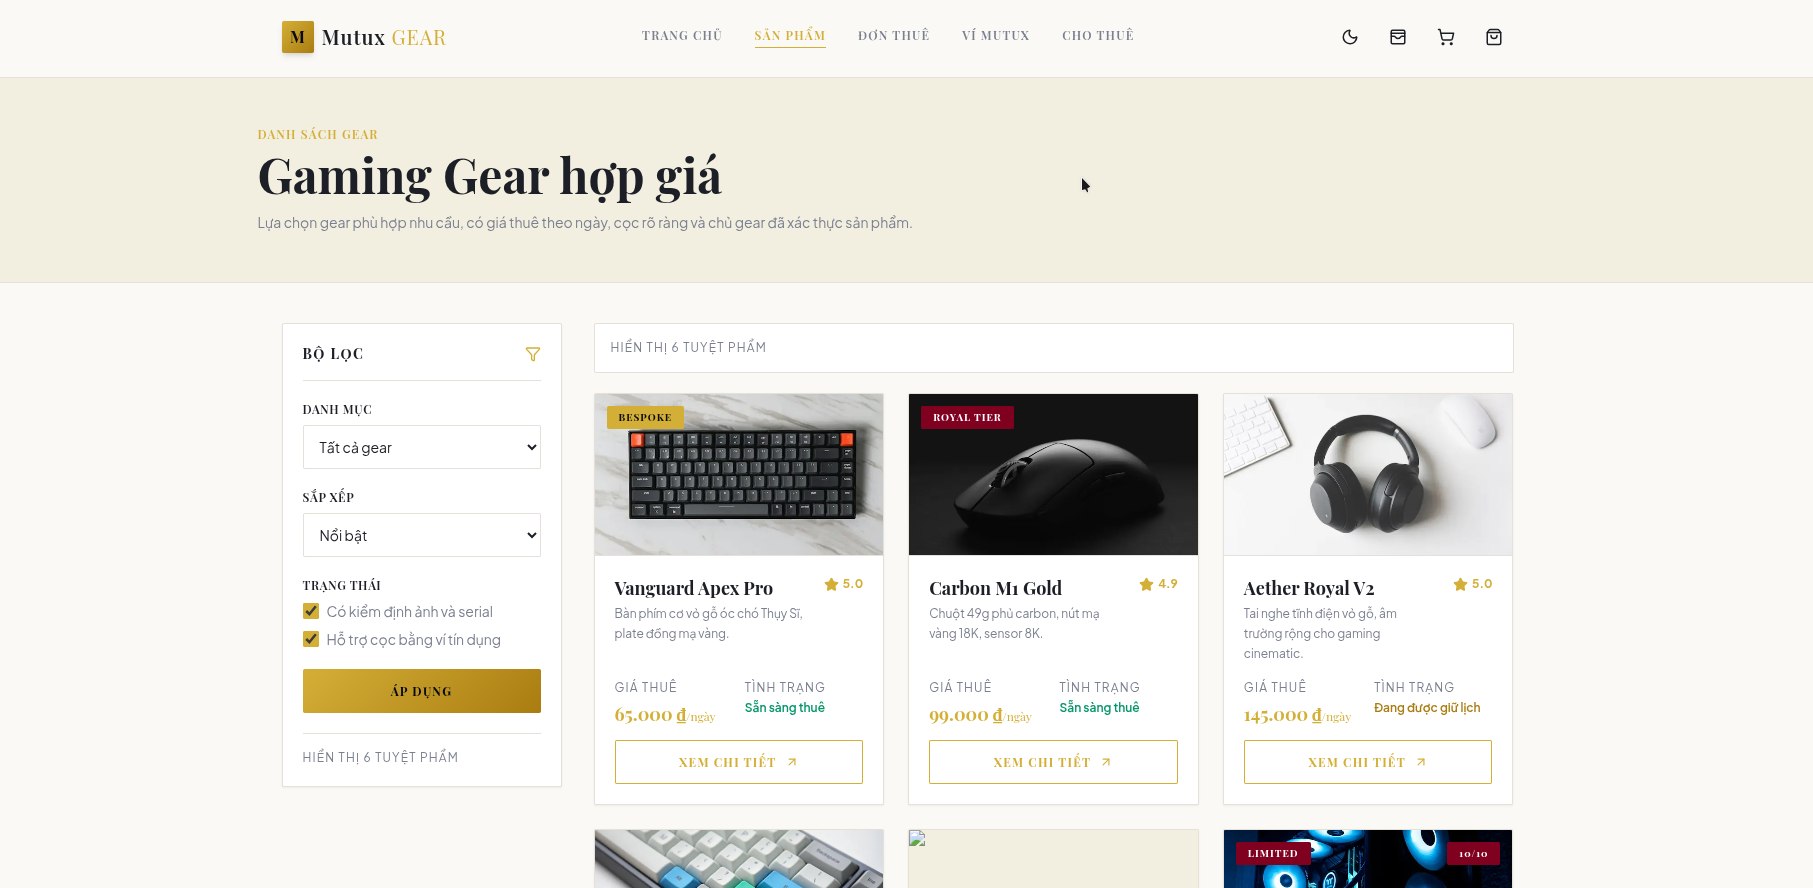
\includegraphics[width=1\textwidth]{PA2/img/mvp/listgear1.png}
    
    \caption{Danh sách sản phẩm trên sàn Mutux}
    \label{fig:my_image}
\end{figure}

Ở tại đây, người dùng có thể filter được theo danh mục mà mình muốn


\begin{figure}[H]
    \centering 
    
    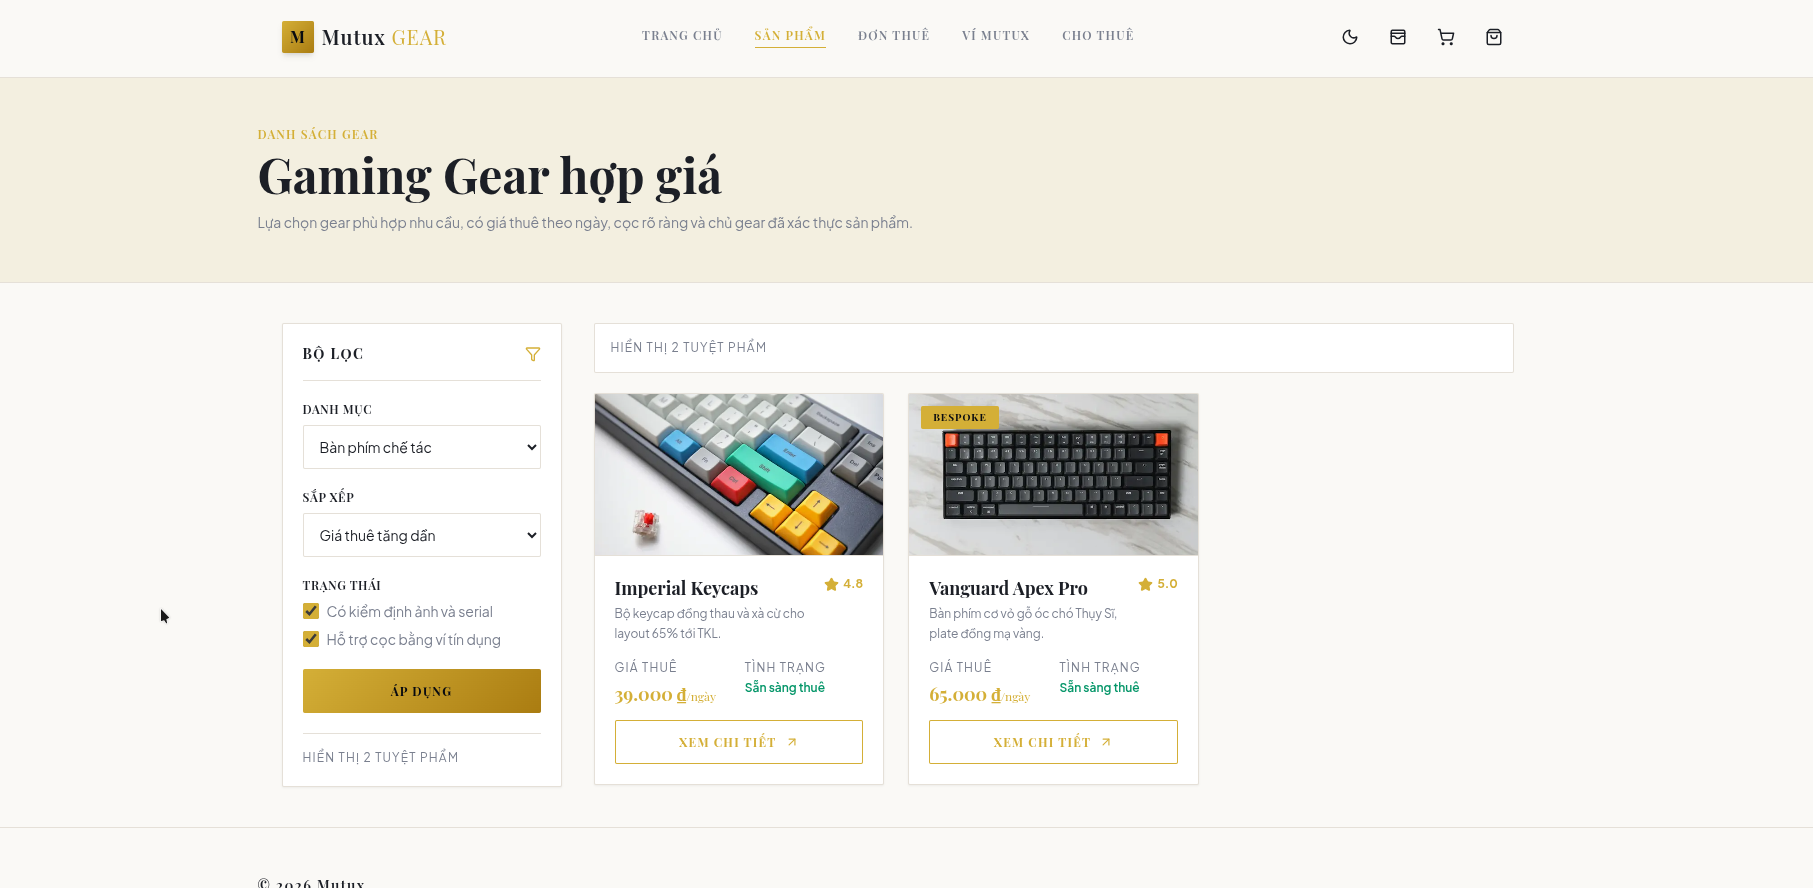
\includegraphics[width=1\textwidth]{PA2/img/mvp/listgear-filter.png}
    
    \caption{Filter theo mục đích của người dùng}
    \label{fig:my_image}
\end{figure}

Sau đó, người muốn thuê chọn sản phẩm mình mong muốn để xem chi tiết

\begin{figure}[H]
    \centering 
    
    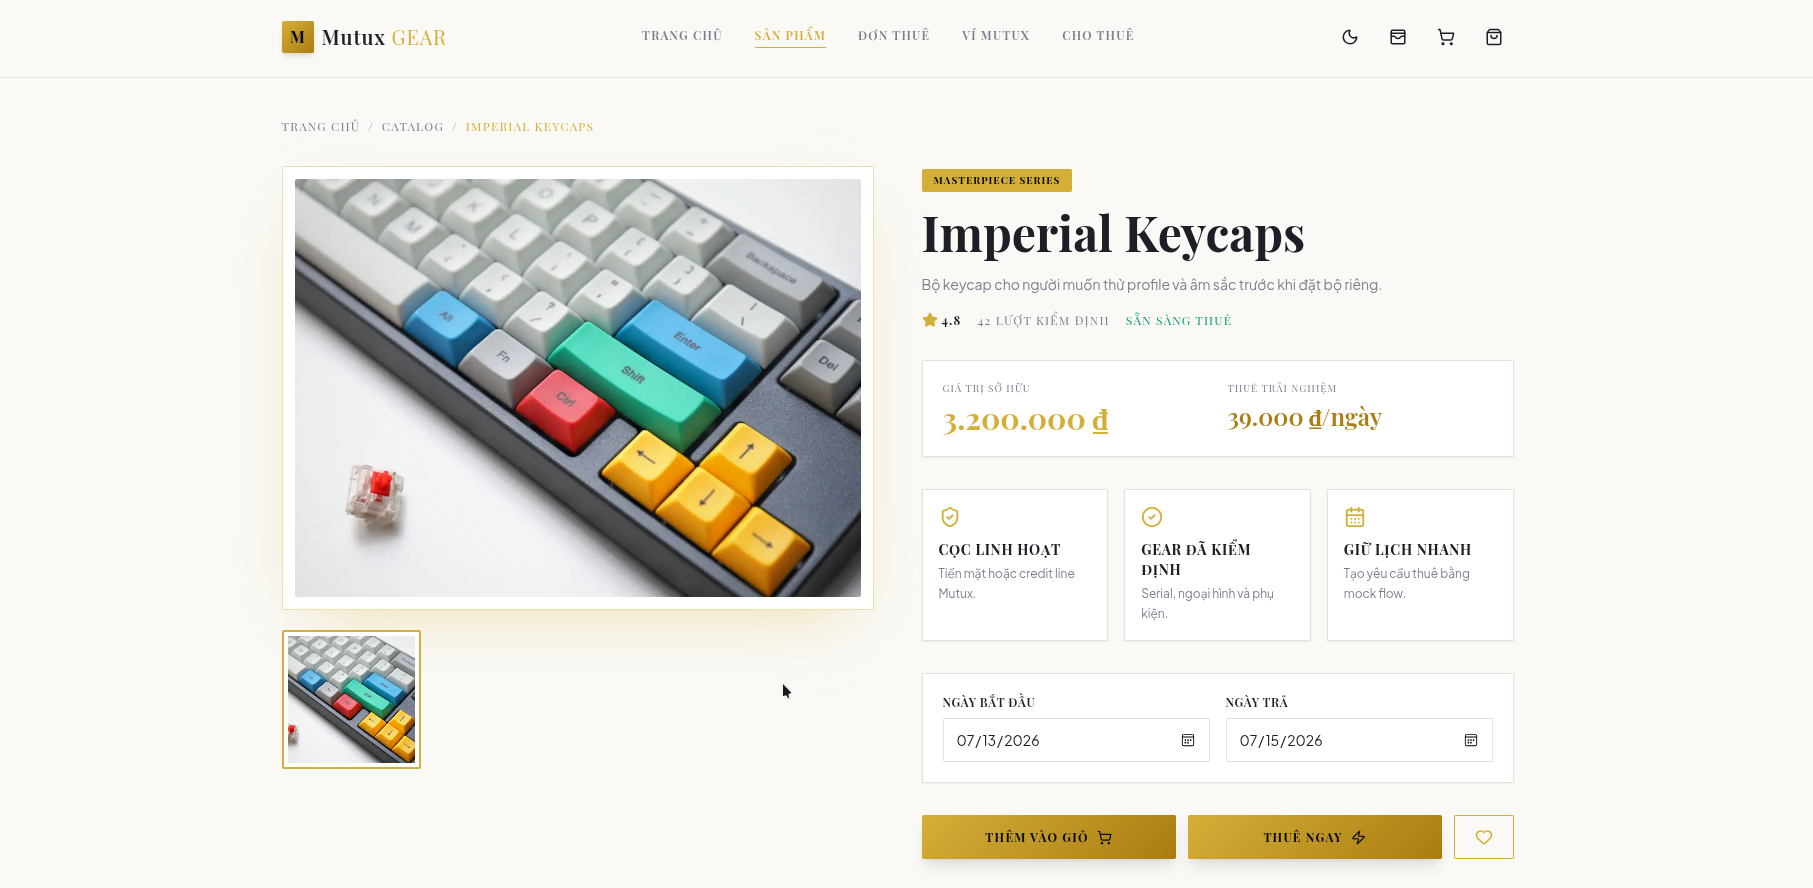
\includegraphics[width=1\textwidth]{PA2/img/mvp/detailgear.png}

    \caption{Trang detail của sản phẩm}
    \label{fig:my_image}
\end{figure}

Tại đây, người dùng có thể chọn ngày bắt đầu đến ngày kết thúc thuê sản phẩm, sau đó, có thể chọn thêm vào giỏ hàng để tiếp tục xem các sản phẩm khác, hoặc tiến hành thanh toán ngay.


\begin{figure}[H]
    \centering 
    
    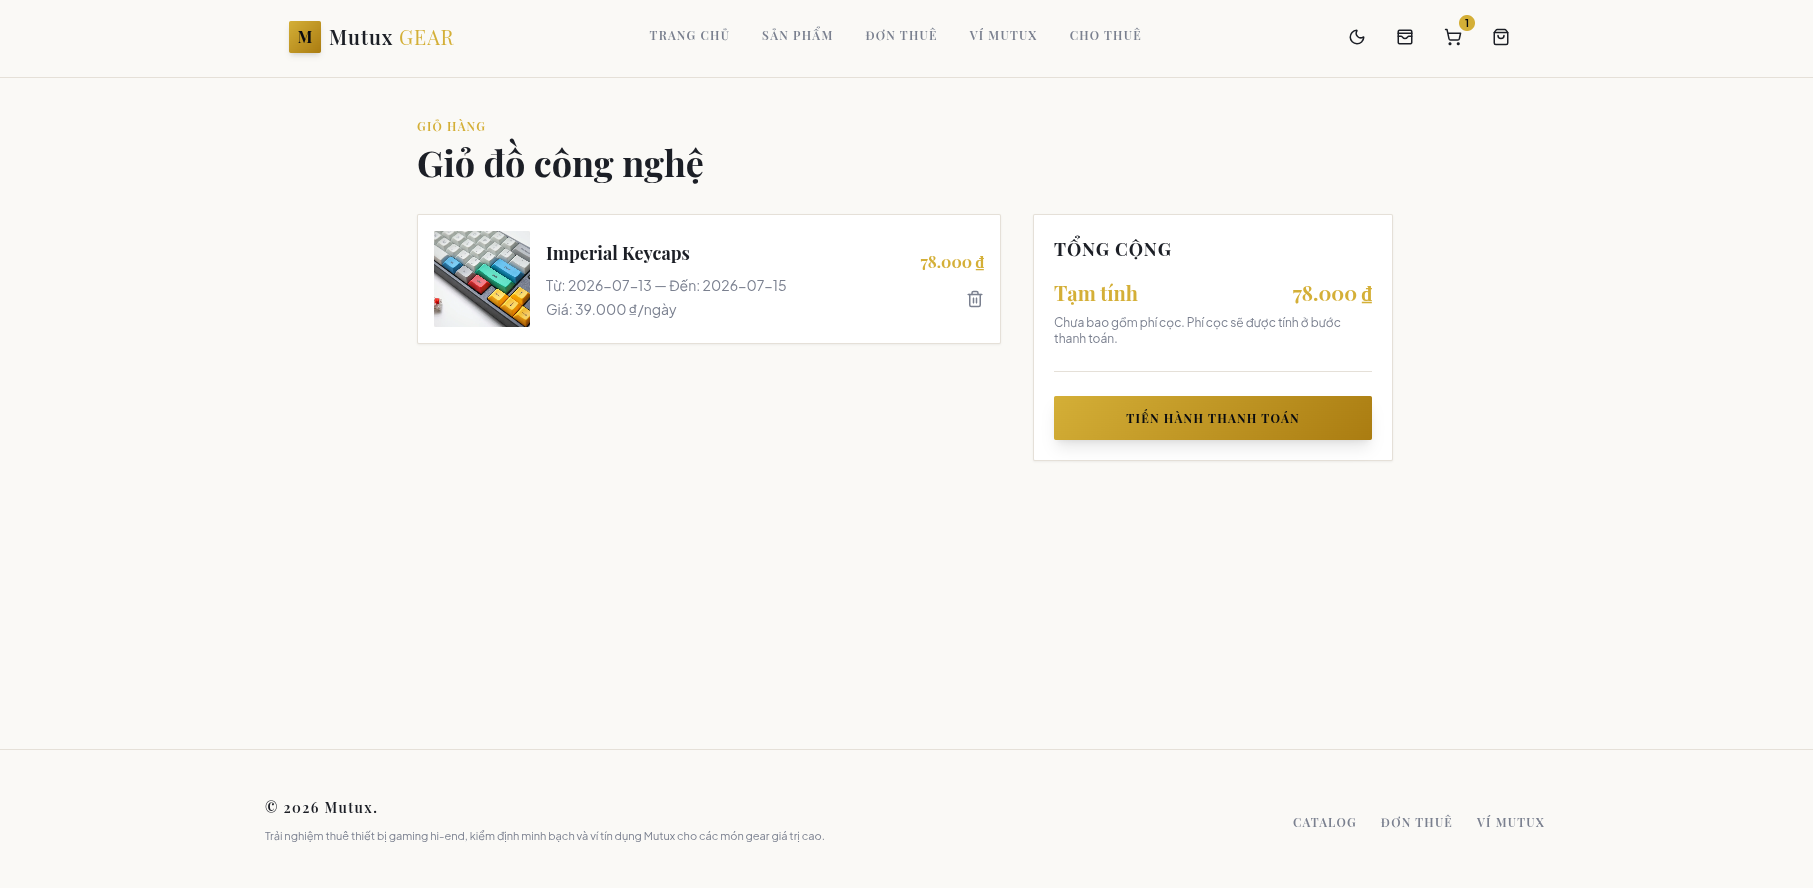
\includegraphics[width=1\textwidth]{PA2/img/mvp/cart.png}

    \caption{Giỏ hàng sản phẩm}
    \label{fig:my_image}
\end{figure}


\begin{figure}[H]
    \centering 
    
    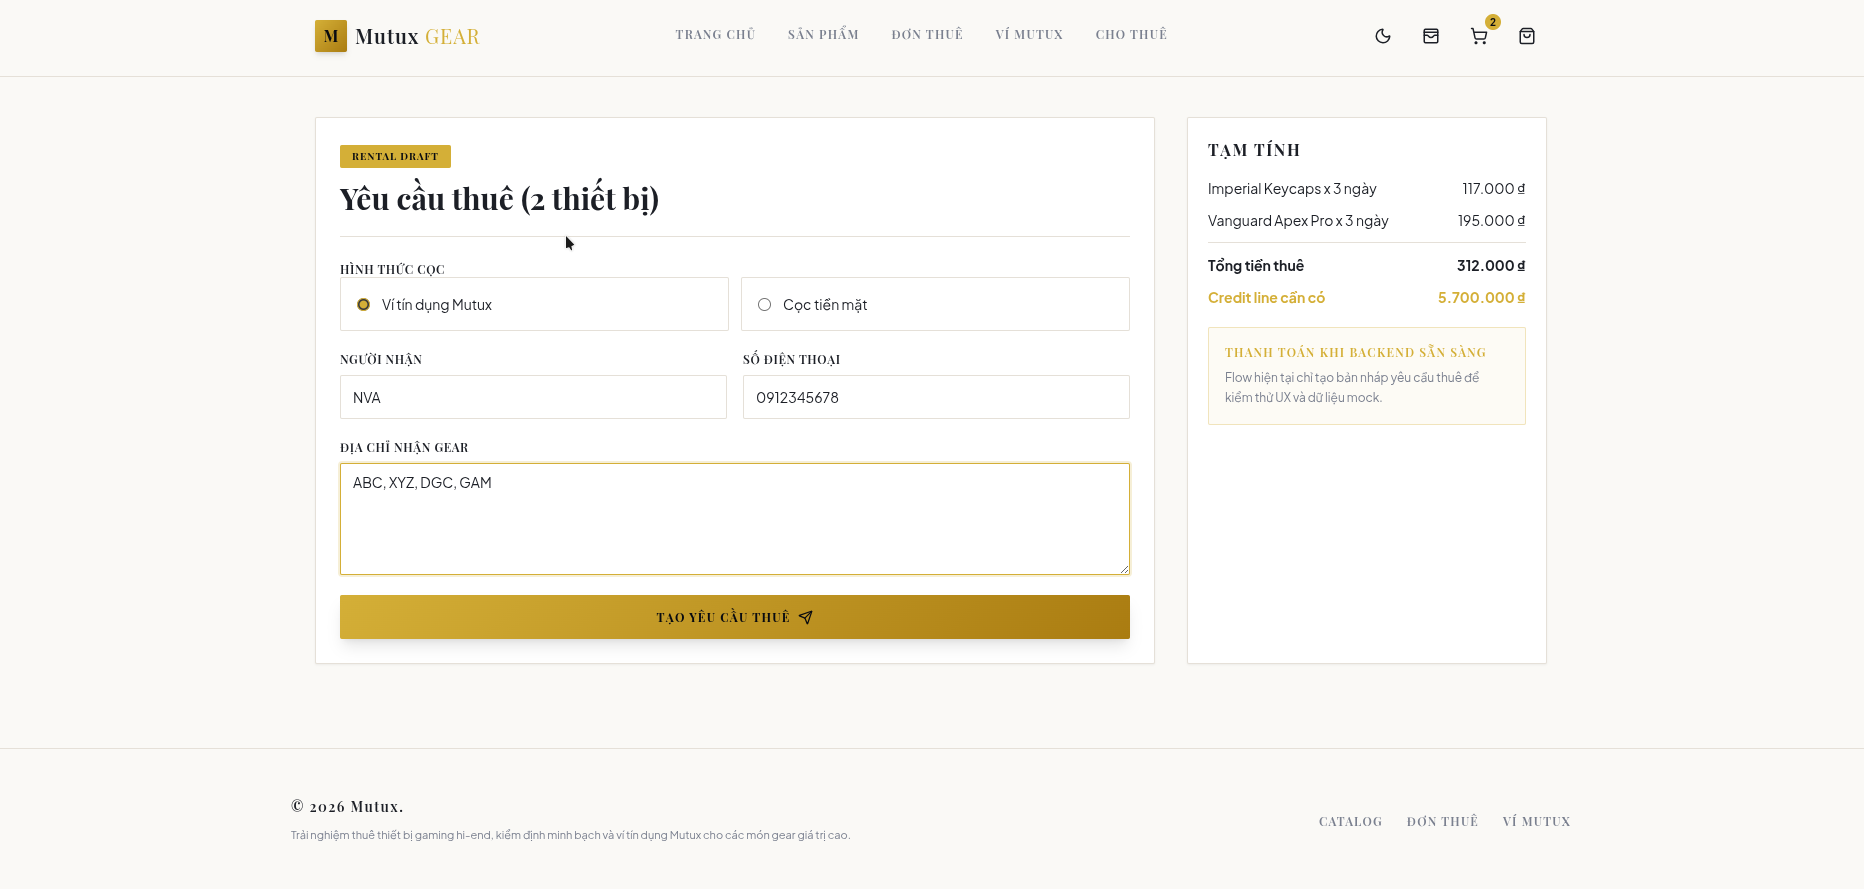
\includegraphics[width=1\textwidth]{PA2/img/mvp/payment.png}

    \caption{Tiến hành thanh toán}
    \label{fig:my_image}
\end{figure}

Tại bước thanh toán, người dùng điền thông tin cá nhân đầy đủ của mình cho việc vận chuyển, bên cạnh đó chọn 2 phương thức thanh toán là cọc theo tiền mặt hoặc cọc theo ví Mutux của hệ thống. Sau khi nhấn \textbf{"Tạo yêu cầu thuê"} thì việc đặt thuê sản phẩm đã kết thúc.

Người dùng sau đó có thể xem các thông tin liên quan đến bản thân như dashboard của ví Mutux hoặc tổng hợp đơn hàng đã đặt
\begin{figure}[H]
    \centering 
    
    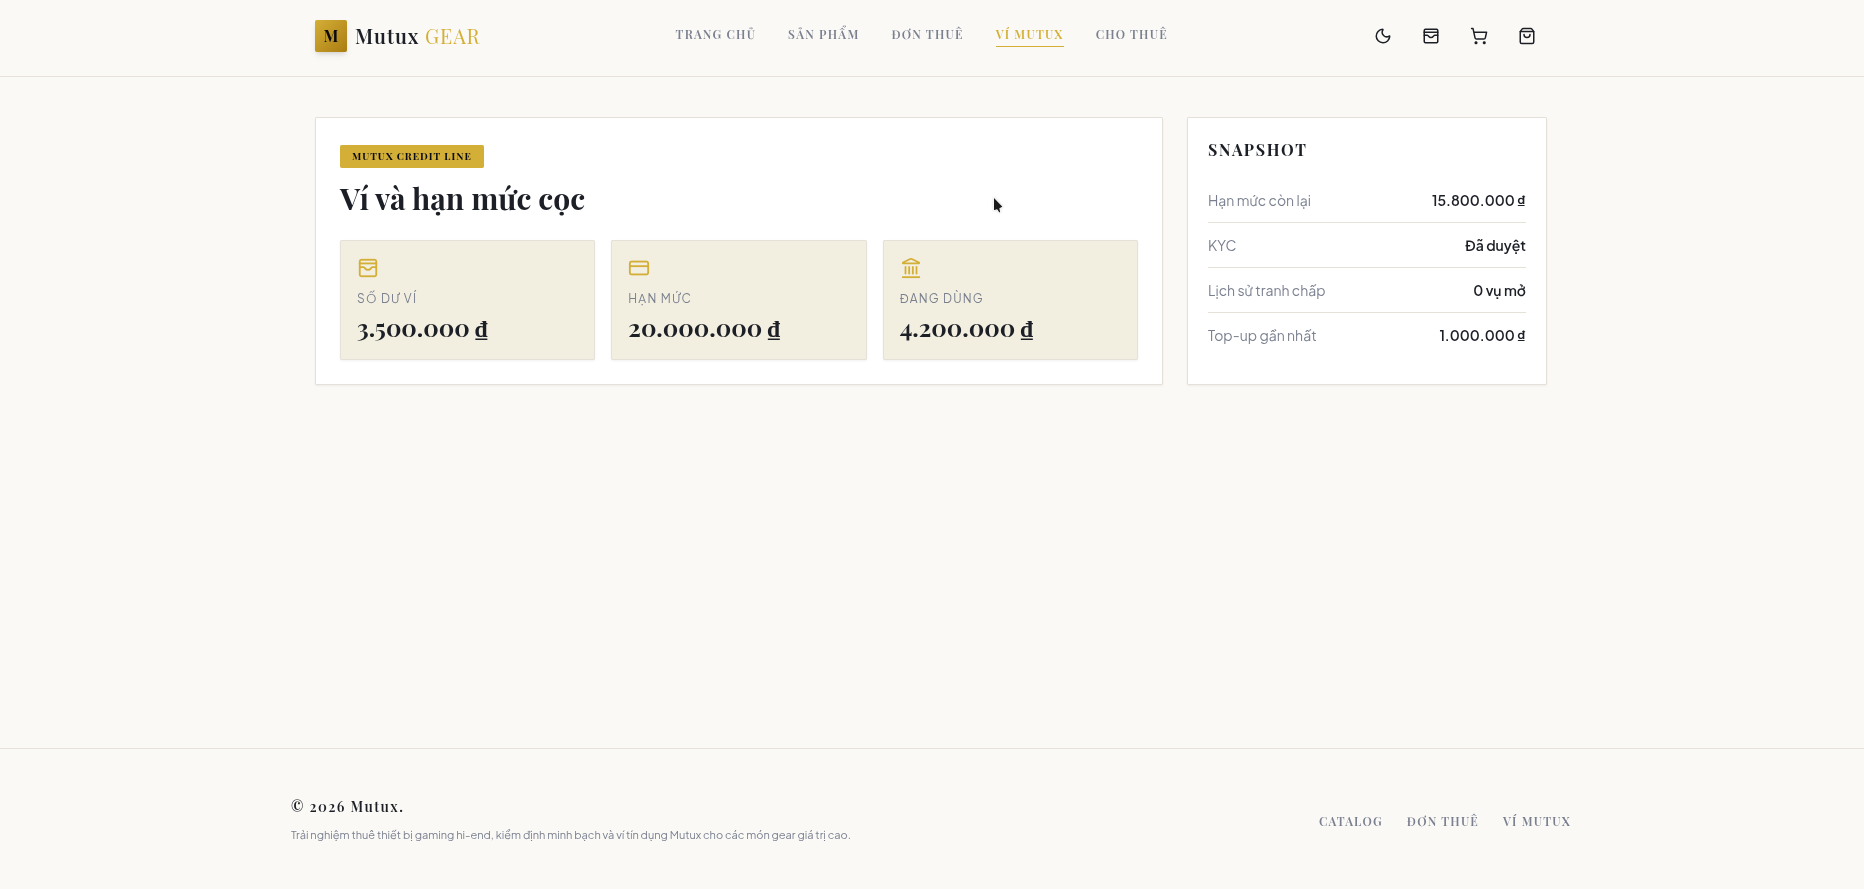
\includegraphics[width=1\textwidth]{PA2/img/mvp/wallet.png}

    \caption{Dashboard quản lý ví Mutux}
    \label{fig:my_image}
\end{figure}


\begin{figure}[H]
    \centering 
    
    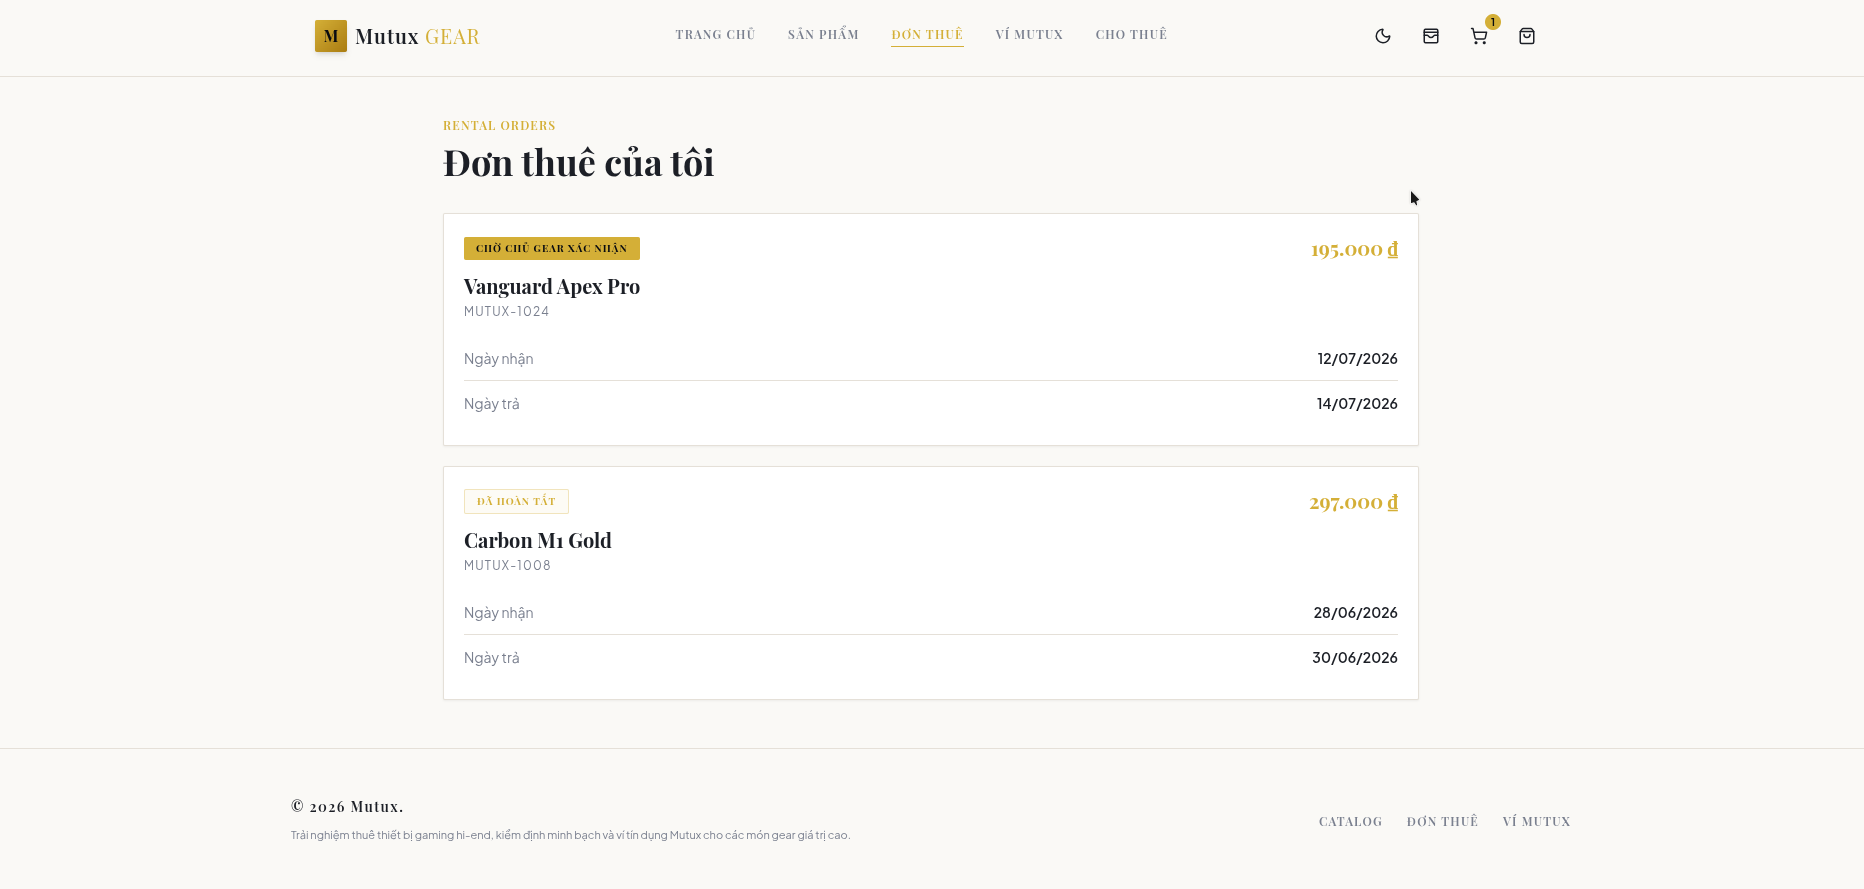
\includegraphics[width=1\textwidth]{PA2/img/mvp/order.png}

    \caption{Tổng hợp đơn hàng đã thực hiện}
    \label{fig:my_image}
\end{figure}

Còn với bên người cho thuê, sau khi đăng nhập thì họ cũng có dashboard riêng để quản lý các thiết bị mình đã đăng lên. Tại đây họ có thể xem hoặc thực hiện các công đoạn liên quan đến CRUD cho các sản phẩm của mình.


\begin{figure}[H]
    \centering 
    
    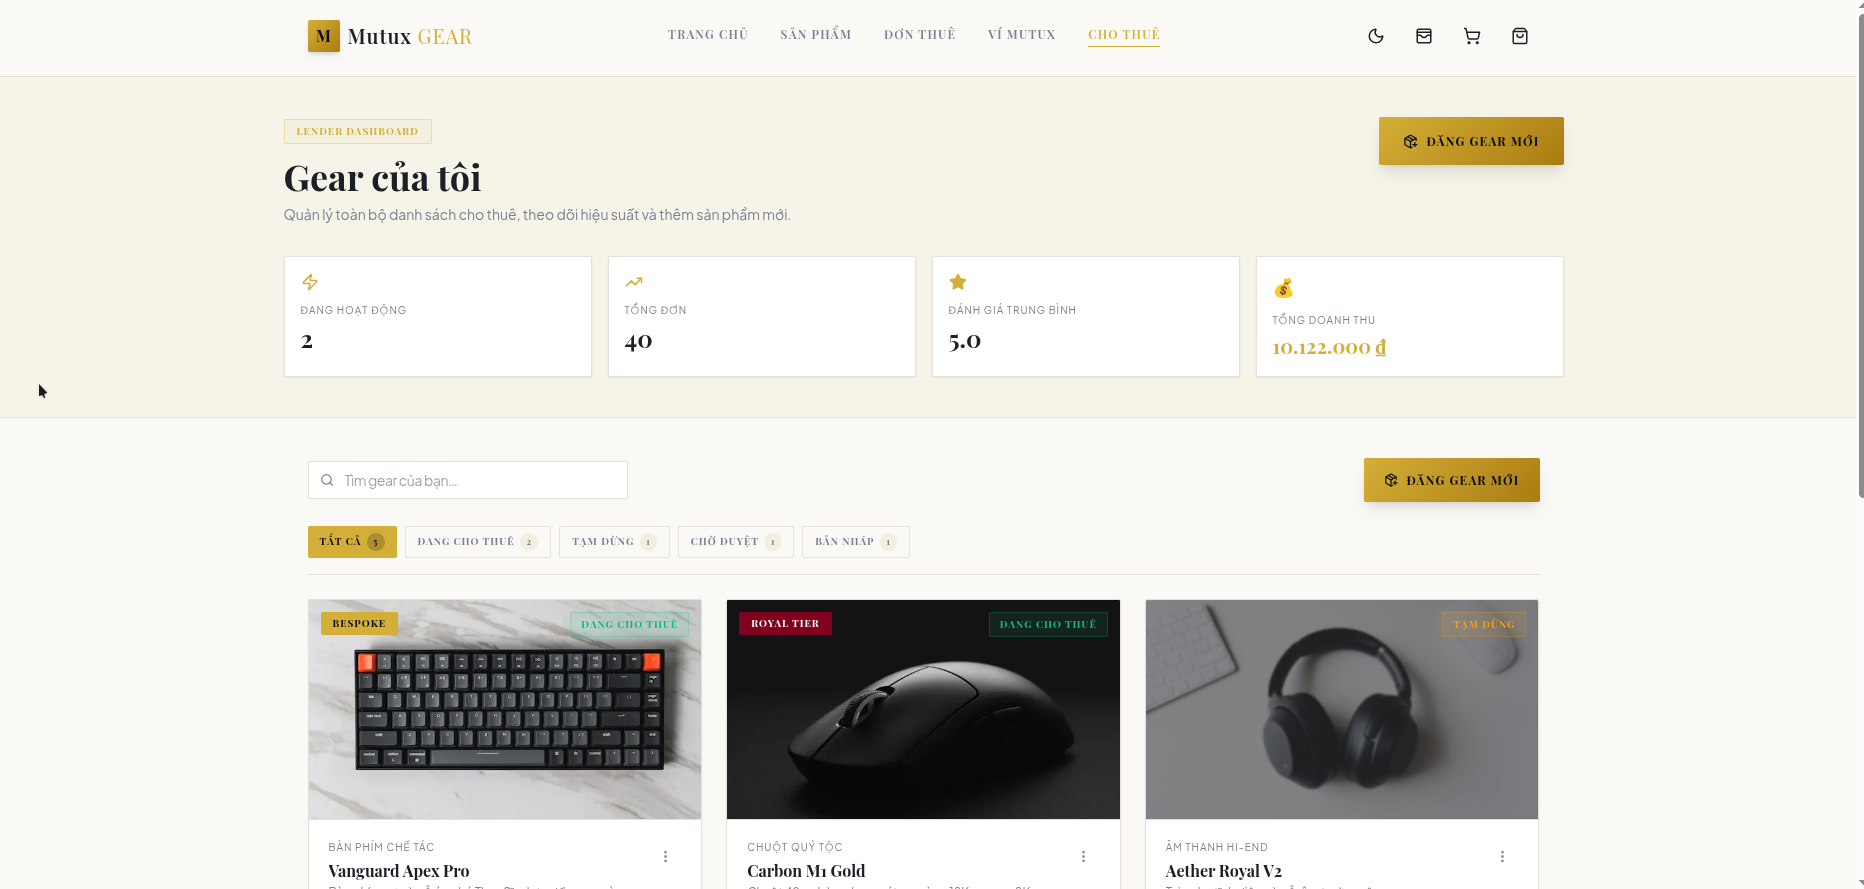
\includegraphics[width=1\textwidth]{PA2/img/mvp/lender-dashboard.png}

    \caption{Dashboard của người cho thuê gear}
    \label{fig:my_image}
\end{figure}


\begin{figure}[H]
    \centering 
    
    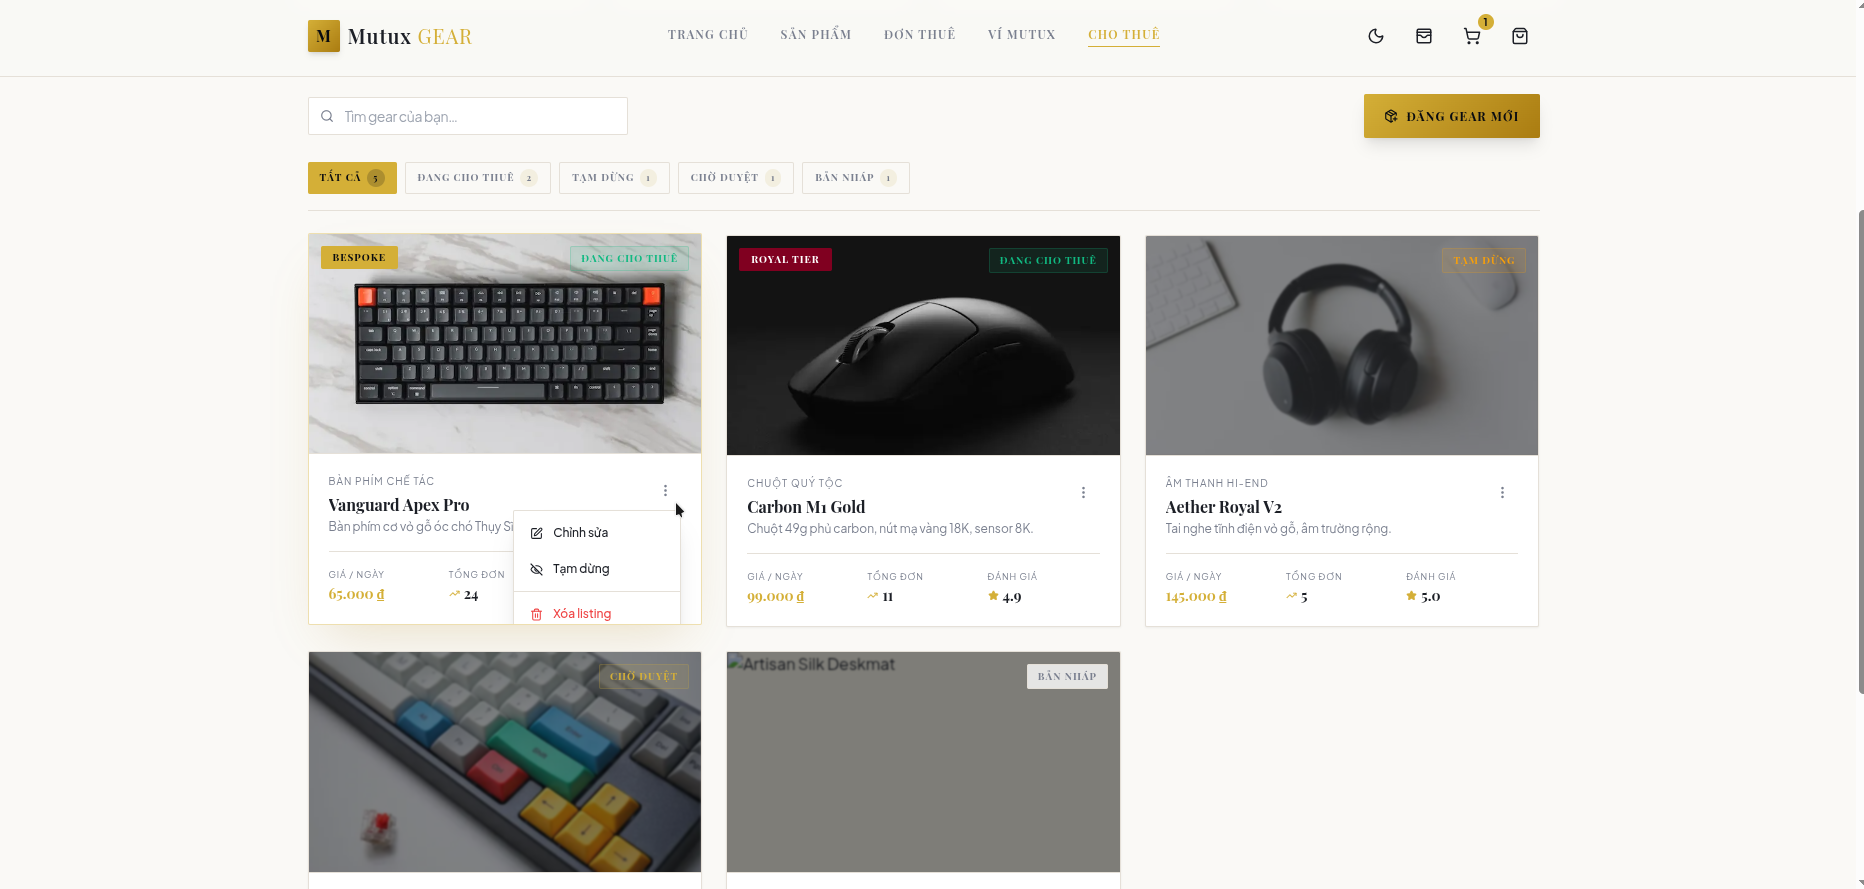
\includegraphics[width=1\textwidth]{PA2/img/mvp/lender crud.png}

    \caption{CRUD sản phẩm đã đăng lên}
    \label{fig:my_image}
\end{figure}


Với sản phẩm mà người cho thuê muốn đăng lên mới, họ sẽ cần hoàn thành form đăng ký sản phẩm như sau:


\begin{figure}[H]
    \centering 
    
    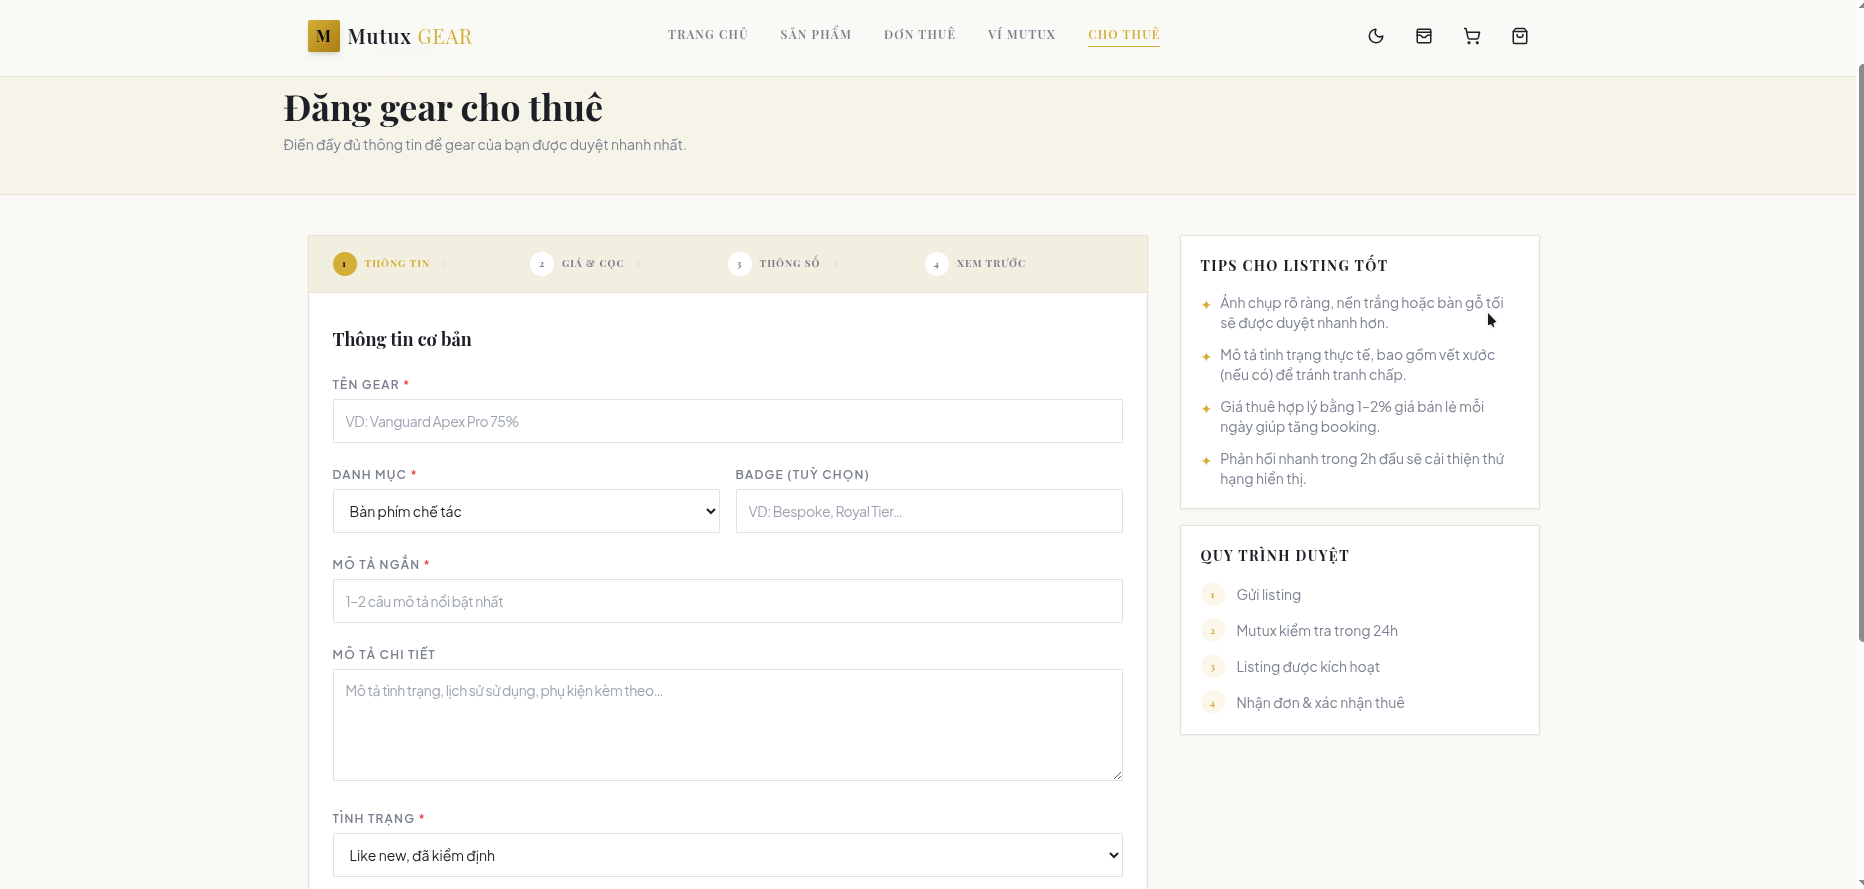
\includegraphics[width=1\textwidth]{PA2/img/mvp/upload gear 1.png}

    \caption{Điền thông tin cơ bản của sản phẩm}
    \label{fig:my_image}
\end{figure}

\begin{figure}[H]
    \centering 
    
    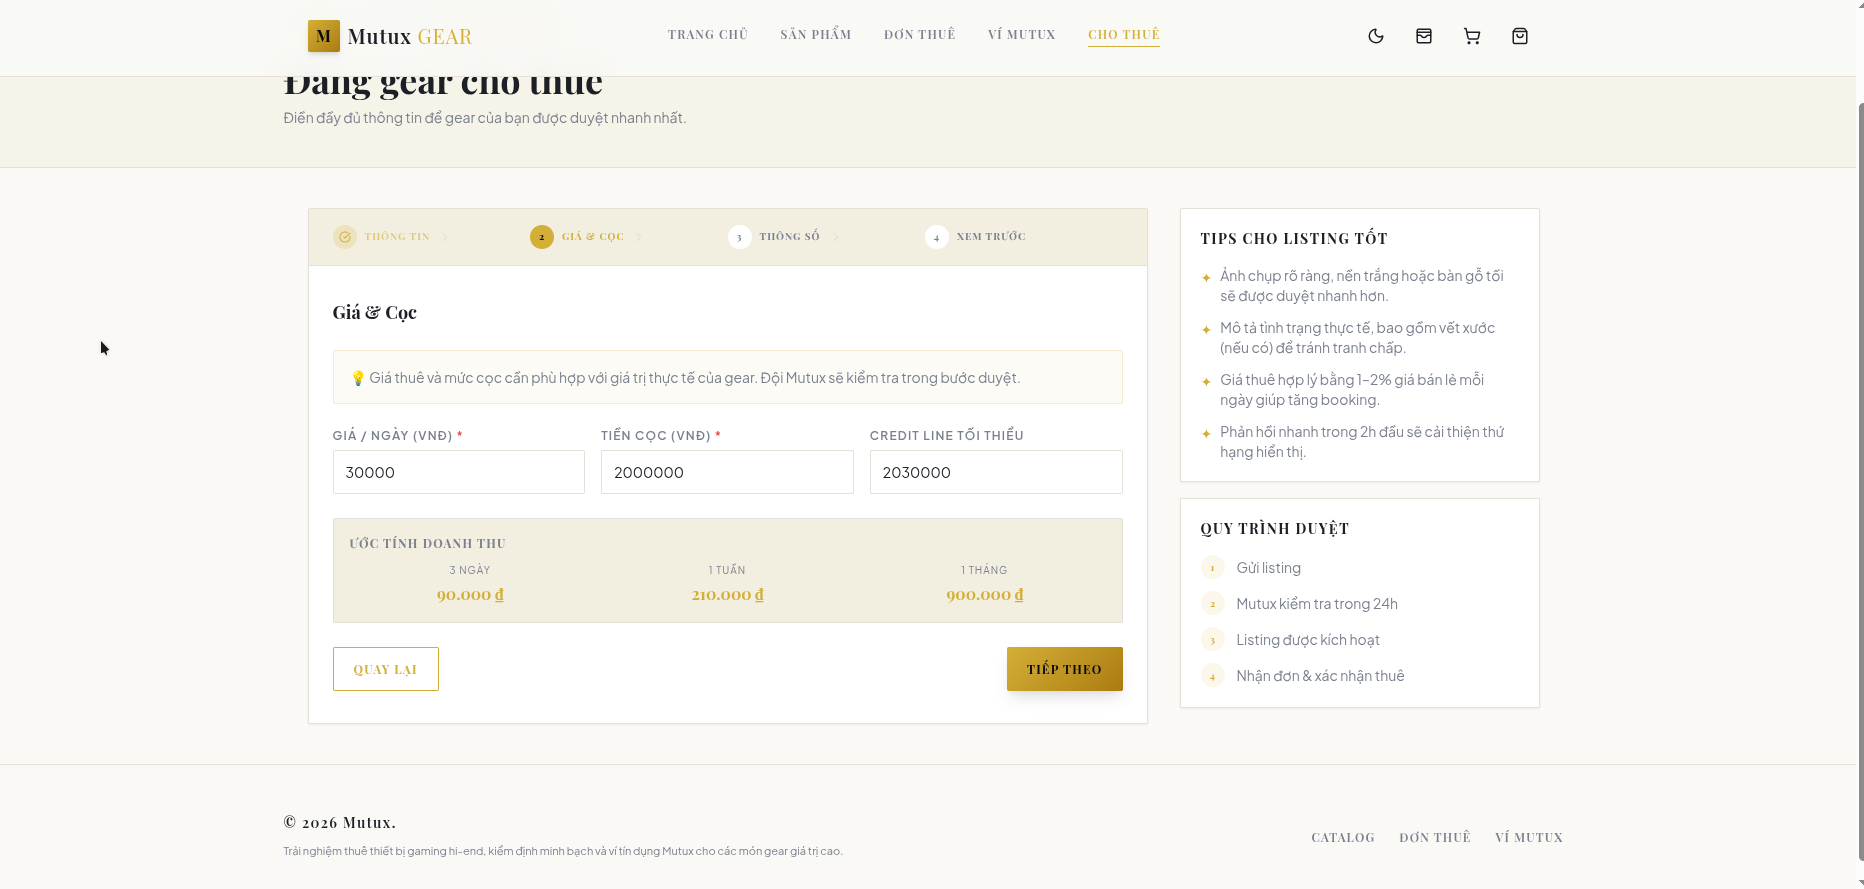
\includegraphics[width=1\textwidth]{PA2/img/mvp/upload gear 2.png}

    \caption{Điền thông tin về giá sản phẩm}
    \label{fig:my_image}
\end{figure}

\begin{figure}[H]
    \centering 
    
    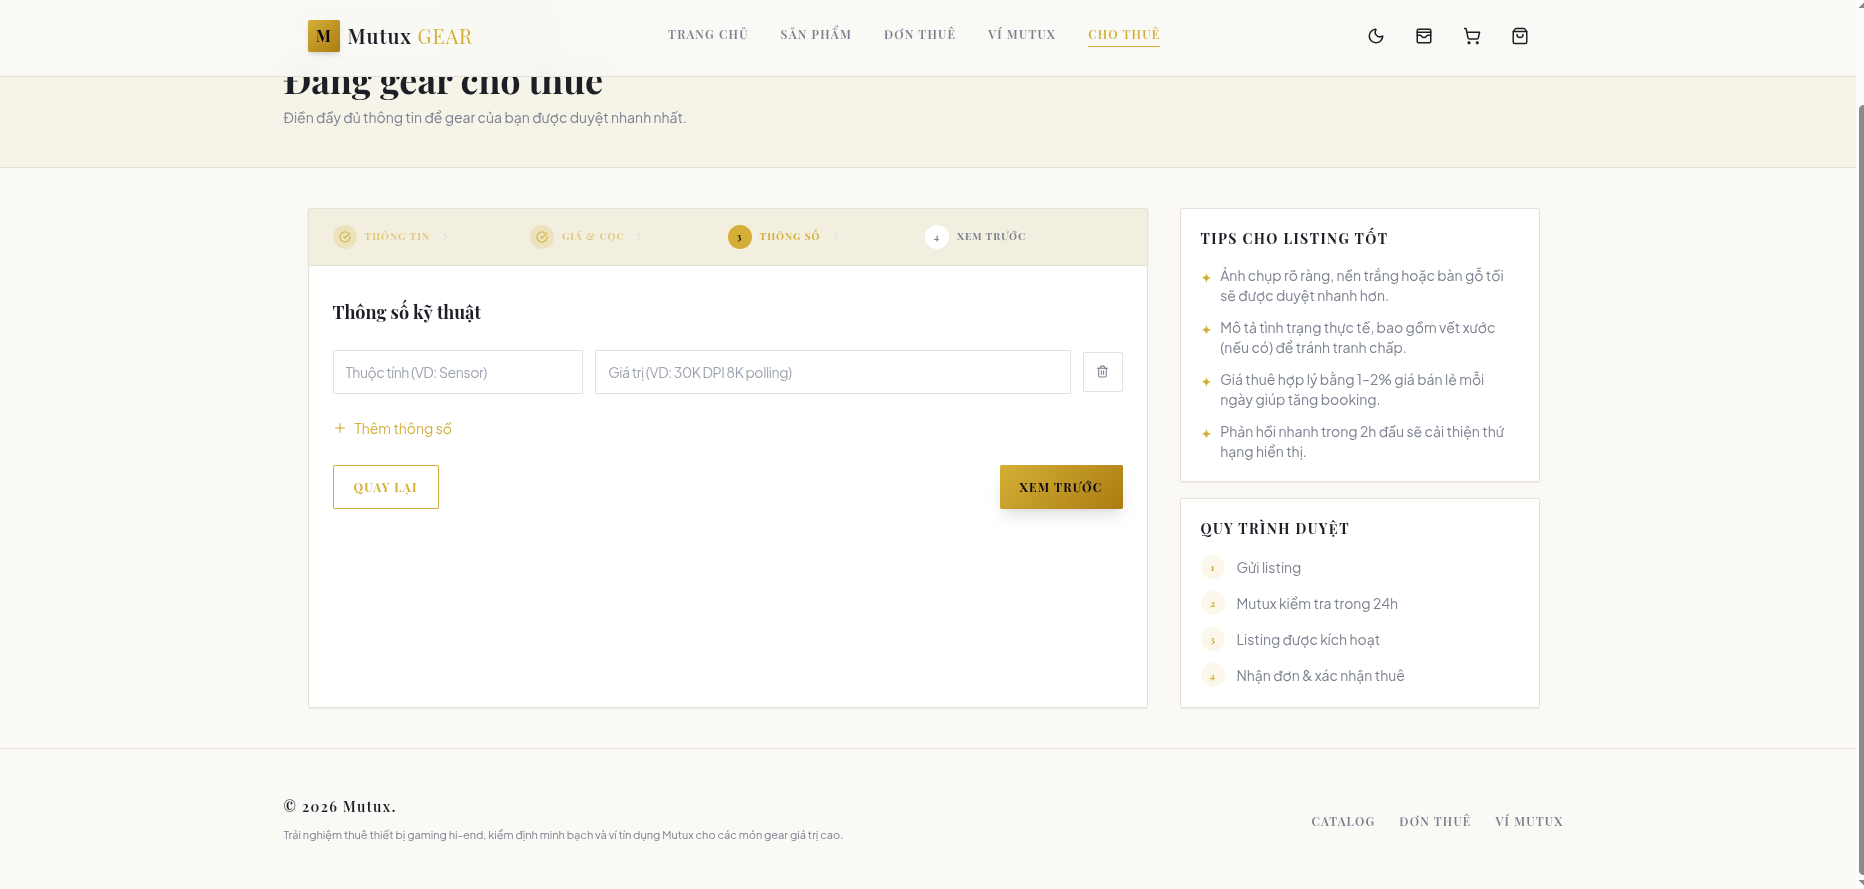
\includegraphics[width=1\textwidth]{PA2/img/mvp/upload gear 3.png}

    \caption{Hoàn thành các thông tin kĩ thuật nếu có}
    \label{fig:my_image}
\end{figure}


\begin{figure}[H]
    \centering 
    
    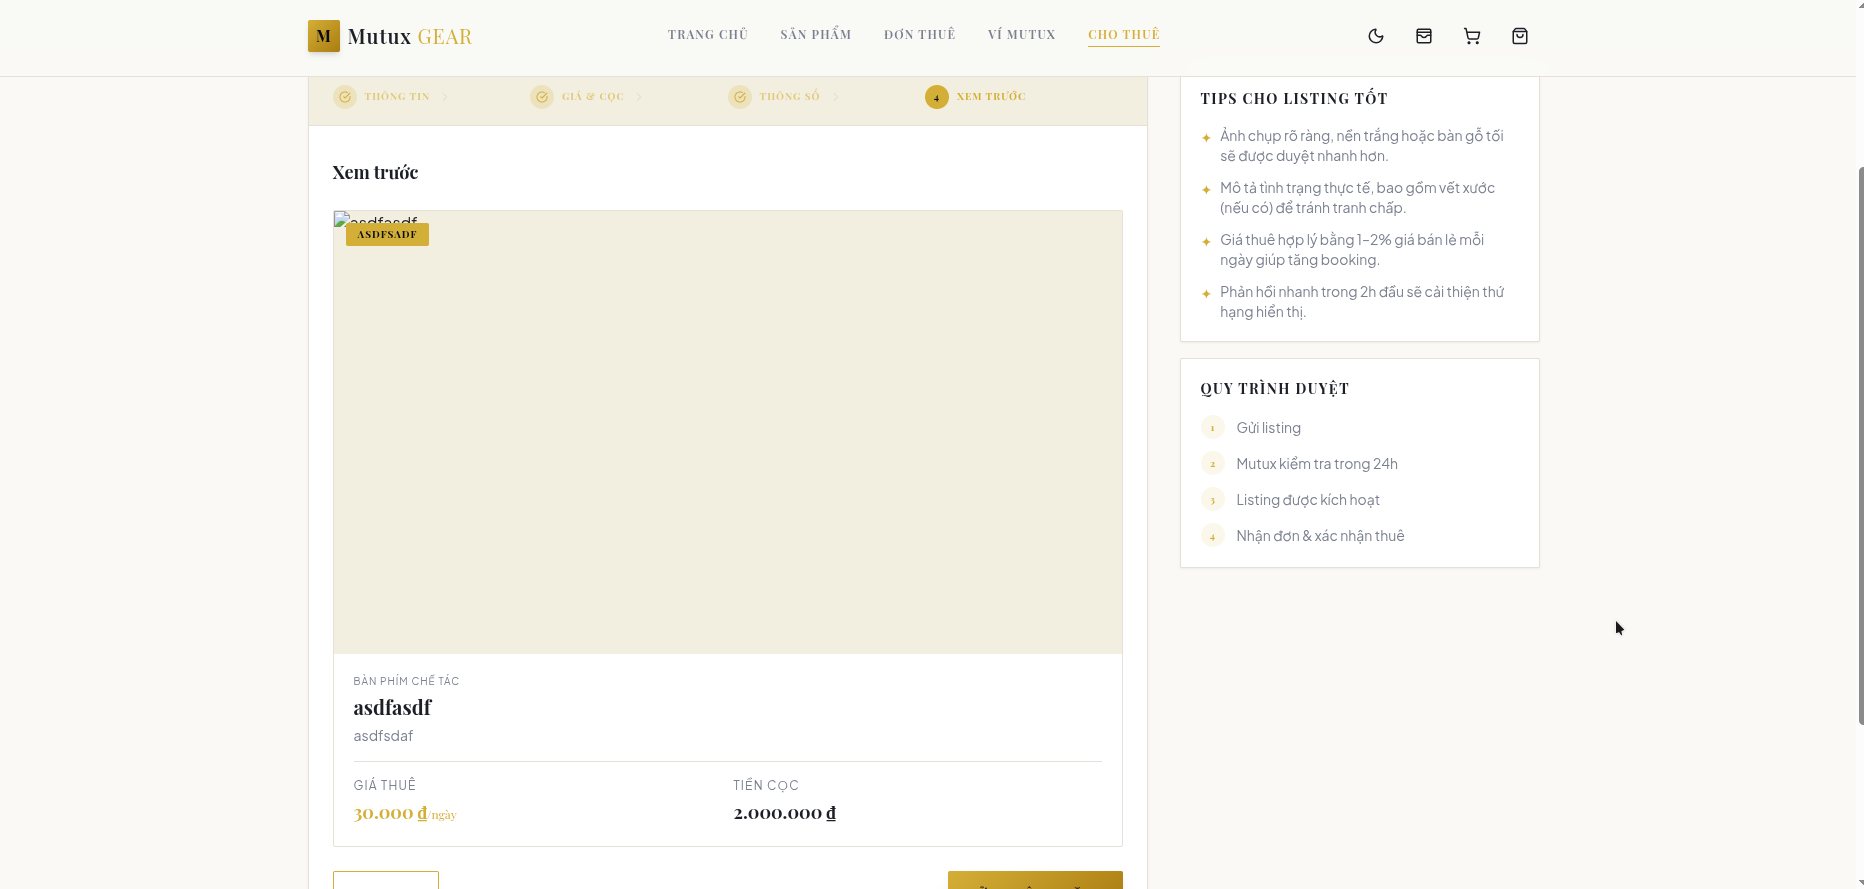
\includegraphics[width=1\textwidth]{PA2/img/mvp/upload gear 4.png}

    \caption{Xem lại sản phẩm mình đã đăng lên}
    \label{fig:my_image}
\end{figure}


\begin{figure}[H]
    \centering 
    
    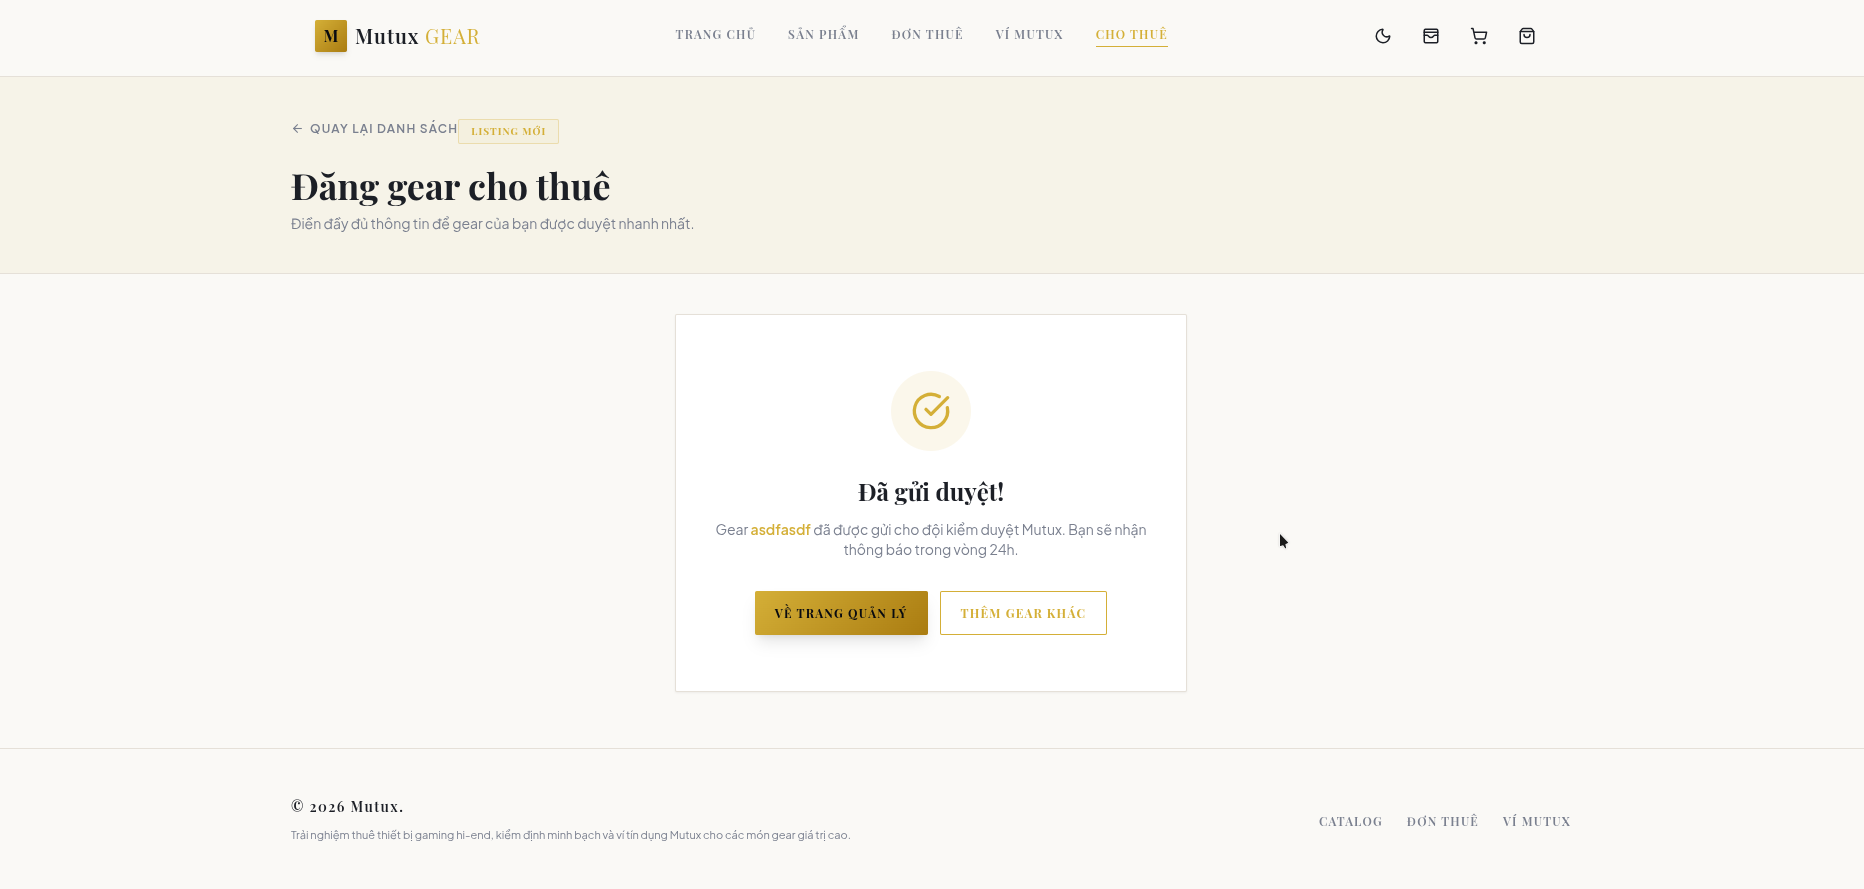
\includegraphics[width=1\textwidth]{PA2/img/mvp/upload gear 5.png}

    \caption{Hoàn thành việc đăng sản phẩm lên sàn}
    \label{fig:my_image}
\end{figure}

Trên đây là UI cơ bản về luồng hoạt động quan trọng của Mutux, các UI quan trọng hơn cùng với MVP hoàn chỉnh sẽ được phát triển trong các giai đoạn tiếp theo.